\section{Achieving fault tolerance with replicated state machines}
\label{motivation:problem}

Consensus algorithms typically arise in the context of
\emph{replicated state machines}~\cite{Schneider:1990}. In this approach, state
machines on a collection of servers compute identical copies of
the same state and can continue operating even if some of the
servers are down.
Replicated state machines are used to solve a variety of
fault tolerance problems in
distributed systems, as described in
Section~\ref{motivation:uses}.
Examples of replicated state machines include Chubby~\cite{Burrows:2006}
and ZooKeeper~\cite{Hunt:2010},
which both provide hierarchical key-value stores for small
amounts of configuration data. In addition to basic operations such as
\emph{get} and \emph{put}, they also provide synchronization primitives
like \emph{compare-and-swap}, enabling concurrent clients to coordinate
safely.

\begin{figure}
\centering
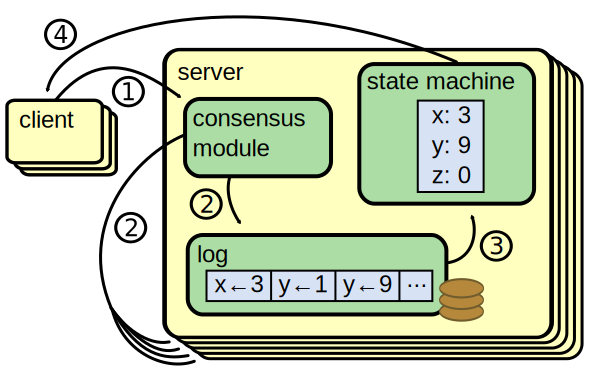
\includegraphics[scale=.50]{motivation/statemachine}
\vcaption[replicated state machine architecture]{
Replicated state machine architecture.
The consensus algorithm
manages a replicated log containing state machine commands from
clients. The state machines process identical sequences of commands
from the logs, so they produce the same outputs.}
\label{fig:motivation:statemachine}
\end{figure}

Replicated state machines are typically implemented using a replicated
log, as shown in Figure~\ref{fig:motivation:statemachine}. Each server stores a log
containing a series of commands, which its state machine executes in order.
Each log contains the same commands in the same order, so each state
machine processes the same sequence of commands. Since the state
machines are deterministic, each computes the same state and the same
sequence of outputs.

Keeping the replicated log consistent is the job of the consensus
algorithm. The consensus
module on a server receives commands from clients and adds them to its log.
It communicates with the consensus modules on other servers to
ensure that every log eventually contains
the same requests in the
same order, even if some servers fail. Once commands are properly
replicated, they are said to be \emph{committed}. Each server's state machine processes
committed commands in log order, and the outputs are returned to clients.
As a result, the servers appear to
form a single, highly reliable state machine.

Consensus algorithms for practical systems typically have the following
properties:
\begin{itemize}
\item They ensure \emph{safety} (never returning an incorrect
result) under all non-Byzantine
conditions, including network delays,
partitions, and packet loss, duplication, and reordering.
\item They are
fully functional (\emph{available}) as long as any majority of the servers are
operational and can communicate with each other and with clients.
Thus, a typical cluster of five servers can tolerate the
failure of any two servers.
Servers are assumed to fail by stopping; they may later recover from
state on stable storage and rejoin the cluster.
\item They do not depend on timing to ensure the consistency
of the logs: faulty clocks and extreme message delays can, at worst,
cause availability problems. That is, they maintain safety under an
\emph{asynchronous} model~\cite{Lynch:1996}, in
which messages and processors proceed at arbitrary speeds.
\item In the common
case, a command can complete as soon as a majority of the cluster
has responded to a single round of remote procedure calls; a minority
of slow servers need not impact overall system performance.
\end{itemize}

